%% abtex2-modelo-artigo.tex, v-1.9.1 laurocesar
%% Copyright 2012-2013 by abnTeX2 group at http://abntex2.googlecode.com/ 
%%
%% This work may be distributed and/or modified under the
%% conditions of the LaTeX Project Public License, either version 1.3
%% of this license or (at your option) any later version.
%% The latest version of this license is in
%%   http://www.latex-project.org/lppl.txt
%% and version 1.3 or later is part of all distributions of LaTeX
%% version 2005/12/01 or later.
%%
%% This work has the LPPL maintenance status `maintained'.
%% 
%% The Current Maintainer of this work is the abnTeX2 team, led
%% by Lauro César Araujo. Further information are available on 
%% http://abntex2.googlecode.com/
%%
%% This work consists of the files abntex2-modelo-artigo.tex and
%% abntex2-modelo-references.bib
%%

% ------------------------------------------------------------------------
% ------------------------------------------------------------------------
% abnTeX2: Modelo de Artigo Acadêmico em conformidade com
% ABNT NBR 6022:2003: Informação e documentação - Artigo em publicação 
% periódica científica impressa - Apresentação
% ------------------------------------------------------------------------
% ------------------------------------------------------------------------

\documentclass[
	% -- opções da classe memoir --
	article,			% indica que é um artigo acadêmico
	11pt,				% tamanho da fonte
	oneside,			% para impressão apenas no verso. Oposto a twoside
	a4paper,			% tamanho do papel. 
	% -- opções da classe abntex2 --
	%chapter=TITLE,		% títulos de capítulos convertidos em letras maiúsculas
	%section=TITLE,		% títulos de seções convertidos em letras maiúsculas
	%subsection=TITLE,	% títulos de subseções convertidos em letras maiúsculas
	%subsubsection=TITLE % títulos de subsubseções convertidos em letras maiúsculas
	% -- opções do pacote babel --
	english,			% idioma adicional para hifenização
	brazil,				% o último idioma é o principal do documento
	sumario=tradicional
	]{abntex2}


% ---
% PACOTES
% ---

% ---
% Pacotes fundamentais 
% ---
\usepackage{lmodern}			% Usa a fonte Latin Modern
\usepackage[T1]{fontenc}		% Selecao de codigos de fonte.
\usepackage[utf8]{inputenc}		% Codificacao do documento (conversão automática dos acentos)
\usepackage{indentfirst}		% Indenta o primeiro parágrafo de cada seção.
\usepackage{nomencl} 			% Lista de simbolos
\usepackage{color}				% Controle das cores
\usepackage{graphicx}			% Inclusão de gráficos
\usepackage{microtype} 			% para melhorias de justificação
% ---
		
% ---
% Pacotes adicionais, usados apenas no âmbito do Modelo Canônico do abnteX2
% ---
\usepackage{lipsum}				% para geração de dummy text
% ---
		
% ---
% Pacotes de citações
% ---
\usepackage[brazilian,hyperpageref]{backref}	 % Paginas com as citações na bibl
\usepackage[alf]{abntex2cite}	% Citações padrão ABNT

\usepackage{color}
% ---

% ---
% Configurações do pacote backref
% Usado sem a opção hyperpageref de backref
\renewcommand{\backrefpagesname}{Citado na(s) página(s):~}
% Texto padrão antes do número das páginas
\renewcommand{\backref}{}
% Define os textos da citação
\renewcommand*{\backrefalt}[4]{
	\ifcase #1 %
		Nenhuma citação no texto.%
	\or
		Citado na página #2.%
	\else
		Citado #1 vezes nas páginas #2.%
	\fi}%
% ---

% ---
% Informações de dados para CAPA e FOLHA DE ROSTO
% ---
\titulo{Uma Visão Ágil sobre o Processo de Desenvolvimento de Software do MPDFT}
\autor{Marcelo Henrique de Oliveira Lima}
\data{2014}
\instituicao{Pós-Graduação em Gestão de TI na Administração Pública}
\local{Brasil}
\orientador{Renato Brown}
% ---

% ---
% Configurações de aparência do PDF final

% alterando o aspecto da cor azul
\definecolor{blue}{RGB}{41,5,195}

% informações do PDF
\makeatletter
\hypersetup{
     	%pagebackref=true,
		pdftitle={\@title}, 
		pdfauthor={\@author},
    	pdfsubject={Modelo de artigo científico com abnTeX2},
	    pdfcreator={LaTeX with abnTeX2},
		pdfkeywords={abnt}{latex}{abntex}{abntex2}{atigo científico}, 
		colorlinks=true,       		% false: boxed links; true: colored links
    	linkcolor=blue,          	% color of internal links
    	citecolor=blue,        		% color of links to bibliography
    	filecolor=magenta,      		% color of file links
		urlcolor=blue,
		bookmarksdepth=4
}
\makeatother
% --- 

% ---
% compila o indice
% ---
\makeindex
% ---

% ---
% Altera as margens padrões
% ---
\setlrmarginsandblock{4cm}{4cm}{*}
\setulmarginsandblock{4cm}{4cm}{*}
\checkandfixthelayout
% ---

% --- 
% Espaçamentos entre linhas e parágrafos 
% --- 

% O tamanho do parágrafo é dado por:
\setlength{\parindent}{1.3cm}

% Controle do espaçamento entre um parágrafo e outro:
\setlength{\parskip}{0.2cm}  % tente também \onelineskip

% Espaçamento simples
\SingleSpacing

% ----
% Início do documento
% ----
\begin{document}

% Retira espaço extra obsoleto entre as frases.
\frenchspacing 

% ----------------------------------------------------------
% ELEMENTOS PRÉ-TEXTUAIS
% ----------------------------------------------------------

%---
%
% Se desejar escrever o artigo em duas colunas, descomente a linha abaixo
% e a linha com o texto ``FIM DE ARTIGO EM DUAS COLUNAS''.
% \twocolumn[    		% INICIO DE ARTIGO EM DUAS COLUNAS
%
%---
% página de titulo
\maketitle

% resumo em português
\begin{resumoumacoluna}

   \textcolor{red}{ESCREVER RESUMO!!!}

   \vspace{\onelineskip}

   \noindent
   \textbf{Palavras-chaves}: Processo Unificado. MPDFT. Métodos Ágeis.
\end{resumoumacoluna}

% ]  				% FIM DE ARTIGO EM DUAS COLUNAS
% ---

% ----------------------------------------------------------
% ELEMENTOS TEXTUAIS
% ----------------------------------------------------------
\textual

% ----------------------------------------------------------
% Introdução
% ----------------------------------------------------------
\section*{Introdução}
\addcontentsline{toc}{section}{Introdução}

\textcolor{red}{ESCREVER INTRODUÇÃO!!!}

\section{Processo Unificado}

Um processo de software é um conjunto de atividades que leva à produção de um
produto de software \cite{sommerville2007}. O Processo Unificado (PU)
\cite{jacobson1999unified} para desenvolvimento de software surgiu como uma
alternativa ao já reconhecidamente ineficiente modelo sequencial ou em cascata.
O modelo em cascata foi o primeiro a ser publicado e teve forte influência dos
processos mais gerais de engenharia de sistema \cite{sommerville2007}. Esse
modelo (cascata) caracteriza-se pelo encadeamento das fases e pelo fato da fase
seguinte não iniciar antes da atual ter terminado. Alguns estudos de
sucesso/falha mostram que projetos que utilizaram o modelo em cascata obtiveram
alta taxa de falha. Acredita-se que esse modelo ganhou forte adoção baseado em
boatos e crenças ao longo dos anos \cite{larman2007utilizando}.

Já o Processo Unificado é fortemente baseado em um modelo
iterativo e incremental. Esse modelo se mostrou mais eficiente em situações que os
requisitos não estão completamente definidos e a entrega de resultados deve ser
antecipada o máximo possível, além de reduzir a quantidade de defeitos.
\citeonline{larman2007utilizando} cita em seu livro que o desenvolvimento
iterativo e evolutivo considera normal que a fase de desenvolvimento comece
antes dos requisitos terem sido definidos em detalhes; a realimentação é usada
para esclarecer e aperfeiçoar as especificações em evolução.

Para fornecer um melhor entendimento sobre o Processo Unificado é comum
dividi-lo em três perspectivas \cite{sommerville2007}:

\begin{enumerate}
   \item Uma perspectiva dinâmica, que mostra as fases do modelo ao longo do
   tempo.
   \item Uma perspectiva  estática, que mostra as atividades realizadas no
   processo.
   \item Uma perspectiva prática, que sugere as boas práticas a serem usadas
   durante o processo.
\end{enumerate}

Conforme citado anteriormente, o Processo Unificado, assim como o modelo
tradicional e vários outros modelos, define um conjunto de fases a serem
seguidas. As quatro principais fases são:

\begin{description}
   \item[1. Concepção] - O objetivo da fase de concepção é estabelecer um
   \textit{business case} para o sistema.
   \item[2. Elaboração] Os objetivos da fase de elaboração são desenvolver um
   entendimento do domínio do problema, estabelecer um framework de arquitetura
   para o sistema, desenvolver o plano de projeto e identificar os riscos
   principais do projeto.
   \item[3. Construção] A fase de construção está essencialmente relacionada ao
   projeto, programação e teste de sistema.
   \item[4. Transição] A fase final do PU está relacionada à transferência do
   sistema da comunidade de desenvolvimento para a comunidade dos usuários e com
   a entrada do sistema em funcionamento no ambiente real.
\end{description}

Apesar das fases do PU se parecerem com as do modelo cascata elas não coincidem
com as atividades do processo e estão mais estritamente ligadas ao negócio do
que a assuntos técnicos \cite{sommerville2007}. Outra característica marcante
da estrutura de fases do PU é que elas podem se sobrepor ao longo do
desenvolvimento, enquanto no modelo tradicional uma fase não inicia antes da
finalização da fase atual.

Outra perspectiva, a estática, é organizada em disciplinas ou fluxos de trabalho
(\textit{workflows}). Uma disciplina é uma sequência de atividades que produz um
resultado de valor observável \cite{Corporation1998}. Por isso a disciplina é a
parte do processo responsável por uma das quatro perguntas básicas de um
processo (quem, o quê, como e quando), o quando. É a disciplina que faz com que
as outras perguntas sejam respondidas no momento adequado do ciclo de vida do
processo. O PU possui nove disciplinas núcleo, seis agrupadas com o título de
engenharia e outras três sob o título de suporte.

\textbf{Disciplinas de Engenharia}

\begin{description}
   \item[1. Modelagem de negócios] - Os processos de negócios são modelados
   usando casos de uso de negócios.
   \item[2. Requisitos] - Os agentes que interagem com o sistema são
   identificados e os casos de uso são desenvolvidos para modelar os requisitos de sistema.
   \item[3. Análise e projeto (design)] - Um modelo de projeto é criado e
   documentado usando modelos de arquitetura, modelos de componente, modelos de
   objeto e modelos de sequência.
   \item[4. Implementação] - Os componentes de sistema são implementados e
   estruturados em subsistemas de implementação.
   \item[5. Teste] - O teste é um processo iterativo realizados em conjunto com
   a implementação.
   \item[6. Implantação] - Uma versão do produto é criada, distribuída aos
   usuários e instalada no local de trabalho.
\end{description}

\textbf{Disciplinas de Apoio/Suporte}

\begin{description}
   \item[1. Gestão de Configuração e Mudança] - Disciplina responsável por
   gerenciar as mudanças do sistema.
   \item[2. Gerência de Projeto] - Disciplina que gerencia o desenvolvimento do
   sistema.
   \item[3. Ambiente] - Disciplina relacionada à disponibilização de ferramentas
   apropriadas de software para a equipe de desenvolvimento.
\end{description}

A terceira perspectiva do Processo Unificado é a prática, que descreve boas
práticas de engenharia de software recomendadas para uso em desenvolvimento de
sistemas \cite{sommerville2007}. São seis:

\begin{description}
   \item[1. Desenvolver software iterativamente] - Planejar os incrementos de
   software com base nas prioridades do cliente e desenvolver e entregar antes
   as características de sistema de maior prioridade no processo de
   desenvolvimento.
   \item[2. Gerenciar requisitos] - Documentar explicitamente os requisitos do
   cliente e manter acompanhamento das mudanças desses requisitos.
   \item[3. Usar arquiteturas baseadas em componentes] - Estruturar a
   arquitetura de sistemas com componentes.
   \item[4. Modelar o software visualmente] - Usar modelos gráficos de UML para
   apresentar as visões estática e dinâmicas do software.
   \item[5. Verificar a qualidade do software] - Garantir que o software atenda
   aos padrões de qualidade da organização.
   \item[6. Controlar as mudanças de software] - Gerenciar as mudanças de
   software, usando um sistema de gerenciamento de mudanças e procedimentos e
   ferramentas de gerenciamento de configuração.
\end{description}

A separação em perpectivas visa dar uma abordagem mais didática, mas o comum é
que elas sejam visualizadas sob uma única ótica, ou seja, na prática as
perspectivas estão sobrepostas conforme Figura \ref{graficodasbaleias}.

\begin{figure}[ht!]
   \centering
   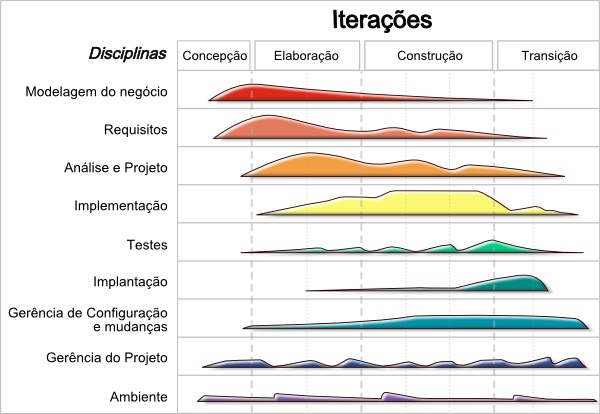
\includegraphics[width=90mm]{graficodasbaleias.jpg}
   \caption{Disciplinas vs Fases}
   \label{graficodasbaleias}
\end{figure}

Essa visão de duas dimensões, para fases e disciplinas, foi uma grande evolução
na forma de desenvolver software, pois enquanto este visa entregar um produto de
trabalho, um artefato, aquele busca atingir um objetivo de desenvolvimento.
Apesar de parecer pouco isso foi uma mudança significativa na forma de escrever
software. O PU proporcionou também um modelo flexível e adaptável que foi base
para muitos outros.

\subsection{MPDFT-UP}

Seguindo recomendações do Tribunal de Conta da União (TCU) presentes no acórdão
nº 1.603/2008 \cite{acordao-tcu-1603-2008} e publicadas no Diário Oficial da União
\cite{dou-20080818}, que visam melhorias na governança de tecnologia da
informação na administração pública federal. No item 9.1.4 desse acórdão é
proposta a utilização de medidas que estimulem a adoção de metodologias de
desenvolvimento de sistemas. Foi feito então um esforço para adequar-se às
recomendações. O Ministério Público do Distrito Federal de Territórios (MPDFT)
desenvolveu um processo denominado MPDFT-UP \cite{mpdft-up}. É um processo
iterativo e incremental baseado no processo unificado. A utilização do PU não é
tão crítica em relação a necessidades e pressões de mercado. Mas, por se tratar
de um órgão público, é necessária especial atenção à documentação dos sistemas
desenvolvidos, formalização de demandas, designação de responsáveis pelo
desenvolvimento e pelos aceites.

Seguindo o entendimento de que não existe um processo ideal várias organizações
desenvolveram abordagens inteiramente diferentes para o desenvolvimento de
software \cite{sommerville2007}.

Os processos evoluíram para explorar as capacidades das pessoas em uma
organização e as características específicas do sistemas que estão sendo
desenvolvidos \cite{sommerville2007}.

Falar sobre as visões implementadas pelo MPDFT-UP. Disciplinas, workflows etc.

\textbf{Etapas que compõem a metodologia de desenvolvimento de sistemas}

\begin{enumerate}
   \item Entendimento inicial
   \item Planejamento e gerência de projeto
   \item Levantamento e análise de requisitos
   \item Implementação e manutenção
   \item Testes
   \item Homologação
   \item Treinamento e implantação
   \item Avaliação
\end{enumerate}

\section{Métodos Ágeis}

Por volta da década de 1990 houve um movimento envolvendo desenvolvedores que
não concordavam com o caminho que estava sendo tomado pelos processos de
software. A burocracia, o peso do processo em detrimento do próprio produto a
ser desenvolvido, o foco nos artefatos que não necessariamente agregam valor,
todos esses fatores foram motivos para a migração que leva a outro extremo, a
redução brusca da burocracia. Tal processo foi tão extremo que levou a criação
de um dos processos de desenvolvimento mais popular do mundo ágil, a programação
extrema (eXtreme Programming - XP) \cite{Beck:1999:ECE:619045.621348}.

Conforme citado por \citeonline{larman2007utilizando}, o PU é completamente
adaptável e aberto a boas práticas de outros metodos. A introdução do PU não
visa diminuir o valor desses outros métodos - muito pelo contrário
\cite{larman2007utilizando}.

http://manifestoagil.com.br/ \cite{agilemanifesto}

\subsection{Scrum}

Scrum das trincheiras.

\subsection{XP}

\subsection{Kanban}

% \subsection{Lean}

% \subsection{Anarchy Programming}

\subsection{Abordagens Ágeis no MPDFT}

    Falta de comprometimento do Product Owner. Em geral, os POs não estão
    interessados ou não têm tempo para lidar com as responsabilidades do papel.
    As dificuldades com a estrutura organizacional. Como o modelo de gestão é
    mais voltado para uma organização matricial, há dificuldades no
    gerenciamento de projetos utilizando técnicas ágeis.

\section{Modelo Híbrido}

Limites bem definidos entre os modelos de processos é algo muito bom do ponto de
vista didático, mas, no mundo prático, é inviável se utilizar somente de um
modelo de desenvolvimento de software. Conforme explicado anteriormente, os
modelos possuem vantagens e desvantagens, o que os tornam interessantes sob
determinadas situações. Contudo, instituições sólidas buscam uma padronização no
modo de trabalho, pois um modo de trabalho uniforme viabiliza o aprimoramento
dos processso de software, no qual a diversidade de processos de software ao
longo da organização é reduzida \cite{sommerville2007}. Isso visa melhorias na
comunicação e redução na curva de aprendizado de novos colaboradores.

Uma vez que o Processo Unificado é bastante flexível e aberto é incentivada a
inclusão de práticas interessantes de outros métodos iterativos tais como:
eXtreming Programming (XP) \cite{Beck:1999:ECE:619045.621348}, Scrum
\cite{schwaber2002agile}

\section{Recomendações}

Grande parte dos problemas relacionados à utilização do Processo Unificado como
base para o desenvolvimento/manutenção de software se deve a tentativa de tornar
um processo já existente em nível executado e às vezes até definido
\textcolor{red}{COLOCAR REFERÊNCIAS PARA NÍVEIS CMMI?} em outro processo, o que
geralmente, e erroneamente, leva a equipe da qualidade a forçar a utilização de
um novo e teoricamente melhor modelo. Assim, em vez de analisar como o software
é tratado em uma organização e simplesmente documentar, a equipe de qualidade
tenta sair de algo executado de forma meramente empírica, em muitos casos, para
algo altamente documentado e, muitas vezes, burocrático. Essa é uma grande
queixa por parte dos envolvidos no uso do processo (funcionários/colaboradores)
e um dos principais responsáveis por um dos grandes mitos envolvendo o PU, o
processo é pesado e, portanto, burocrático.



Apoio à projetização
do órgão.

Melhorias na gestão de configuração: políticas de controle de versão e estilo de
código.

Melhorias no fluxo do processo: liberar casos de uso para desenvolvimento e
teste. Posteriormente, liberar o roteiro de teste para o desenvolvimento.

Abordagem mais agilista.

Incentivo ao desenvolvimento  orientado a teste.

Definições de tecnologias e arquitetura.

Melhorias no processo de arquitetura. Incluir prova de conceito no fluxo dos
projetos.

% Finaliza a parte no bookmark do PDF, para que se inicie o bookmark na raiz
% ---
\bookmarksetup{startatroot}% 
% ---

% ---
% Conclusão
% ---
\section*{Considerações finais}
\addcontentsline{toc}{section}{Considerações finais}

Adotar de maneira mais direta as outras disciplinas do PU.

A gestão de configuração e mudança é fundamental para a padronização do processo
e redução na curva de aprendizado.

Padronização dos repositórios de projetos. Ex.: gerencia, requisitos, projeto,
implementação, teste, design etc.

Criação de uma política de gestão de configuração.

Encoding padrão.

Ajustes/melhorias na estrutura organizacional para facilitar a adoção de
métodos ágeis. Equipes mais projetizadas.

Definição de tecnologias suportadas.

Definições de arquitetura e de uma possível arquitetura de referência.

% ----------------------------------------------------------
% ELEMENTOS PÓS-TEXTUAIS
% ----------------------------------------------------------
\postextual

% ----------------------------------------------------------
% Referências bibliográficas
% ----------------------------------------------------------
\bibliography{abntex2-modelo-references}

\end{document}
